\chapter{Half Wave Rectification}
	\section{Aim}
		\begin{itemize}
			\tightlist
			\item Explain Rectification
			\item Explain Half Wave Rectification
			\item Explain Half Wave Rectification:For Positive Half Cycle
			\item Explain Half Wave Rectification:For Negative Half Cycle
		\end{itemize}

	\section{Apparatus}
		\begin{itemize}
			\tightlist
			\item Silicon/Germanium Diode
			\item Resistor
			\item AC Power Source
			\item Oscilloscope
		\end{itemize}
	
	\section{Theory}
		\subsection{Rectification}
			\begin{figure}[h]
				\centering
				
\includegraphics[width=0.9\linewidth]{img/exp6/1}
				\caption{Function of a Rectifier}
				\label{fig:rffxn}
			\end{figure}
			A rectifier is a device that converts alternating current (AC) to direct current (DC), a process known as rectification. Rectifiers are essentially of two types – a half wave rectifier and a full wave rectifier.
			
		\subsection{Half Wave Rectification}
			\begin{figure}[h]
				\centering
				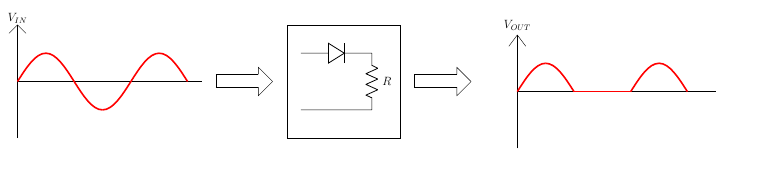
\includegraphics[width=0.9\linewidth]{img/exp6/2}
				\caption{Half Wave Rectification}
				\label{fig:rfhw}
			\end{figure}
			On the positive cycle the diode is forward biased and on the negative cycle the diode is reverse biased. By using a diode we have converted an AC source into a pulsating DC source. In summary we have ‘rectified’ the AC signal.
			\begin{figure}[h]
				\centering
				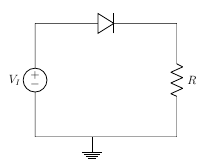
\includegraphics[width=0.3\linewidth]{img/exp6/3}
				\caption{Half Wave Rectification Circuit}
				\label{fig:rfhwc}
			\end{figure}
			The simplest kind of rectifier circuit is the half-wave rectifier.The half-wave rectifier is a circuit that allows only part of an input signal to pass. The circuit is simply the combination of a single diode in series with a resistor, where the resistor is acting as a load.
		
		\subsection{Half Wave Rectifiers – Waveforms}
			\begin{figure}[h]
				\centering
				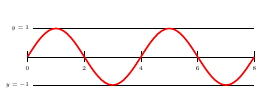
\includegraphics[width=0.7\linewidth]{img/exp6/6}
				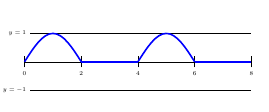
\includegraphics[width=0.7\linewidth]{img/exp6/4}
				\caption{Half Wave Rectification Wave Form}
				\label{fig:rfhwwf}
			\end{figure}
			The output DC voltage of a half wave rectifier can be calculated with the following two ideal equations.			
			$$V_{peak}=V_{rms} \times \sqrt{2}$$
			$$V_{dc}=\frac{V_{peak}}{\pi}$$
		
		\subsection{Half Wave Rectification: For Positive Half Cycle}
			\begin{figure}[h]
				\centering
				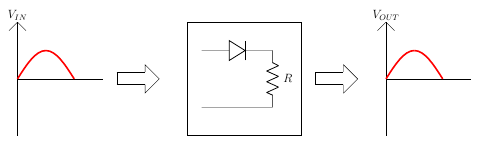
\includegraphics[width=0.9\linewidth]{img/exp6/5}
				\caption{Half Wave Rectification - Positive Half Cycle}
				\label{fig:rfhwphc}
			\end{figure}			
			Diode is forward biased, acts as a short circuit, passes the waveform through.
			
			For positive half cycle: $$V_I - V_b - I \times r_d - I \times R=0$$ where,
			$V_I$ is the input voltage,\\
			$V_b$ is barrier potential,\\
			$r_d$ is diode resistance,\\
			$I$ is total current,\\
			$R$ is resistance\\
			$$I=\frac{V_I - V_b}{r_d + R}$$
			$$V_O = I \times R$$
			$$V_O =\frac{V_I - V_b}{r_d + R} \times R$$
			For $r_d << R$,
			$$V_O = V_I- V_b$$
			$V_b$ is 0.3 for Germanium ,
			$V_b$ is 0.7 for Silicon
			
			For $V_I<V_b$,
			
			The diode will remain OFF.The Output voltage will be,
			$$V_O =0$$
			For $V_I>V_b$,
			
			The diode will be ON.The Output voltage will be,
			$$V_O = V_I- V_b$$
		
		\subsection{Half Wave Rectification: For Negative Half Cycle}
			\begin{figure}[h]
				\centering
				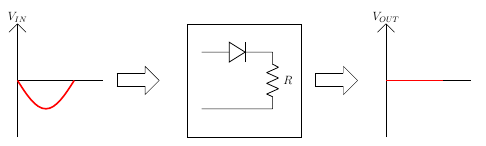
\includegraphics[width=0.9\linewidth]{img/exp6/7}
				\caption{Half Wave Rectification - Negative Half Cycle}
				\label{fig:rfhwnhc}
			\end{figure}
			Diode is reverse biased, acts as a open circuit, does not pass the waveform through.
			
			For negative half cycle:
			$$V_O=0 \quad Since, \quad I =0$$
		
		\subsection{Half wave Rectification: For an Ideal Diode}
			For Ideal Diode,
			$$V_b = 0$$
			For positive half cycle,
			$$V_O = V_I$$
			For negative half cycle,
			$$V_O = 0$$
			
		\subsection{Average output voltage}	
			\begin{align*}
				V_O &= \begin{cases} 
					V_m \sin wt, \quad\quad 0 \leq wt \leq \pi\\
					0, \quad\quad\quad\quad\quad \pi \leq wt \leq 2 \pi
				\end{cases}\\
				V_{av} &= \frac{V_m}{\pi} =0.318V_m
			\end{align*}
		
		\subsection{RMS load voltage}			
			$$V_{rms}=I_{rms} \times R = \frac {V_m}{2}$$
		
		\subsection{Average load current}
			\begin{align*}
				I_{av} &= \frac{V_{av}}{R} =\frac{\frac{V_m}{\pi}}{R}\\
				I_{av} &= \frac{V_{m}}{\pi \times R}=\frac{I_m}{\pi}
			\end{align*}
		
		\subsection{RMS load current}			
			$$I_{rms}=\frac {I_m}{2}$$
			
		\subsection{Form factor}
			It is defined as the ratio of rms load voltage and average load voltage.
			\begin{align*}					
				F.F &= \frac{V_{rms}}{V_{av}}\\
				&= \frac{\frac{V_{m}}{2}}{\frac{V_{av}}{2}}=\frac{\pi}{2}=1.57
			\end{align*}
			$$F.F \geq 1$$
			$$rms \geq av$$
		
		\subsection{Ripple Factor}			
			\begin{align*}
				\gamma &= \sqrt{{F.F}^2-1} \times 100\%\\
				&= \sqrt{{1.57}^2-1} \times 100\%\\
				&= 1.21\%
			\end{align*}		
		\subsection{Efficiency}
			It is defined as ratio of dc power available at the load to the input ac power.
			\begin{align*}
				n\% &= \frac{P_{load}}{P_{in}} \times 100\%\\
				&= \frac {{I_{dc}^2} \times R}{{I_{rms}^2} \times R}\times 100\%\\
				&= \frac{\frac {I_{m}^2}{\pi^2}}{\frac{I_{m}^2}{4}}\times 100\%\\
				&= \frac{4}{\pi^2}\times 100\%\\
				&= 40.56 \%
			\end{align*}
	
		\subsection{Peak Inverse Volatge}
			For rectifier applications, peak inverse voltage (PIV) or peak reverse voltage (PRV) is the maximum value of reverse voltage which occurs at the peak of the input cycle when the diode is reverse-biased.The portion of the sinusoidal waveform which repeats or duplicates itself is known as the cycle. The part of the cycle above the horizontal axis is called the positive half-cycle, the part of the cycle below the horizontal axis is called the negative half cycle. With reference to the amplitude of the cycle, the peak inverse voltage is specified as the maximum negative value of the sine-wave within a cycle's negative half cycle.
							
			
			$$ V_{PIV}=V$$
			$$ -V_m +V=0 \Rightarrow V=V_m$$
			$$ V_{PIV} \geq V_m$$
	
	\section{Procedure}
		\begin{enumerate}
			\tightlist
			\item Set the resistor $R_L$.
			\item Click on 'ON' button to start the experiment.
			\item Click on 'Sine Wave' button to generate input waveform
			\item Click on 'Oscilloscope' button to get the rectified output.
			\item Vary the Amplitude, Frequency, volt/div using the controllers.
			\begin{figure}[h]
				\centering
				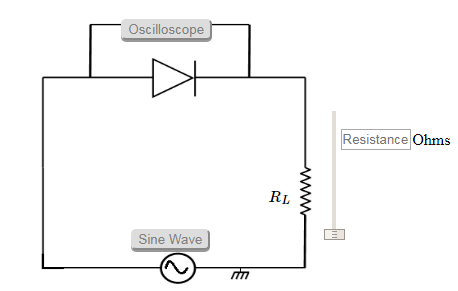
\includegraphics[width=0.7\linewidth]{img/exp6/8}
				\caption{}
				\label{fig:rfhwp}
			\end{figure}
			\item Click on "Dual" button to observe both the waveform.
			\item Channel 1 shows the input sine waveform, Channel 2 shows the output rectified waveform.
			\item Calculate the Ripple Factor.Theoretical Ripple Factor= 1.21.
		\end{enumerate}
	
	\section{Calculations}	
		Measure the $V_m$
		
		$$V_{rms}= \frac{V_m}{2}$$
		$$V_{dc}= \frac{V_m} {\pi}$$
		Ripple Factor($RP$)$$RP = \frac{V_{ac}}{V_{dc}}$$
		Since, $$V_{ac}=\sqrt{(V^2_{rms}-V^2_{dc})}$$		
		Peak Current: $0.74999999 mA$
		
	\section{Observations}
		\begin{figure}[h]
			\centering
			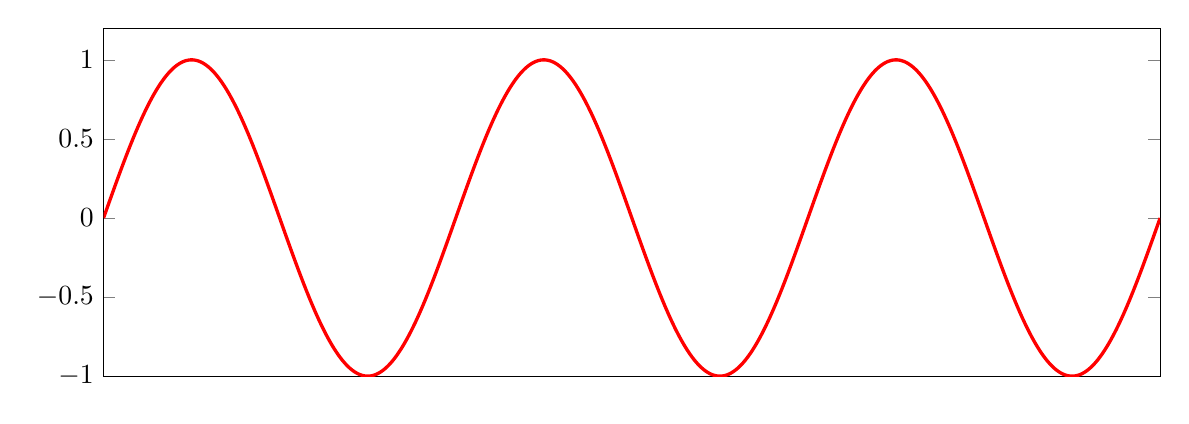
\begin{tikzpicture}
				\begin{axis}[
					domain=0:3*360,
					samples=4*360,
					xtick=\empty,
					width=15cm, height=6cm,
					ymin=-1,
					enlarge x limits=false
					]
					\addplot [red, very thick] {sin(x)};
				\end{axis}
			\end{tikzpicture}
			\caption{Un-Rectified AC Waveform}
		\end{figure}
		\begin{figure}[h]
			\centering
			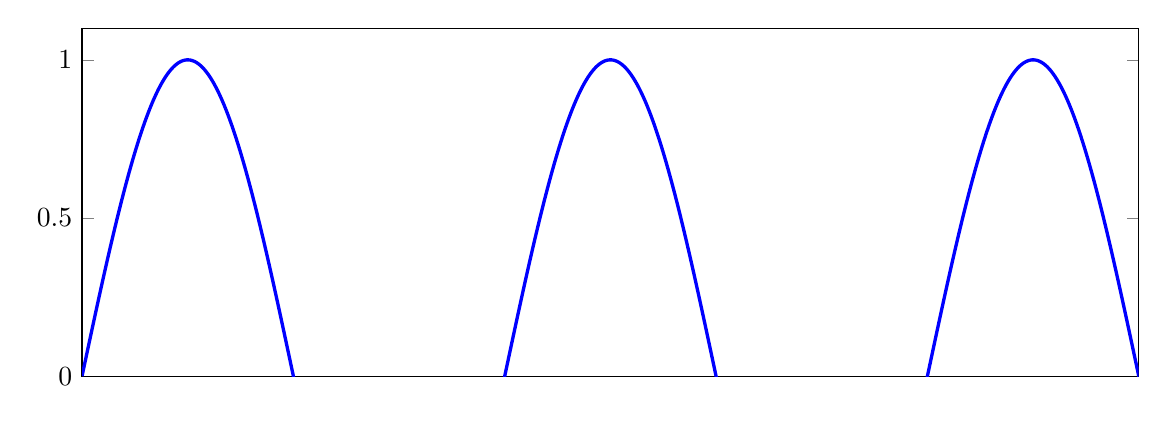
\begin{tikzpicture}
				\begin{axis}[
					domain=0:3*360,
					samples=4*360,
					xtick=\empty,
					width=15cm, height=6cm,
					ymin=0,
					enlarge x limits=false
					]
					\addplot [blue, very thick] {sin(x)};
				\end{axis}
			\end{tikzpicture}
			\caption{Half Wave Rectified Waveform}
		\end{figure}
	
	\section{Result}
		A rectifier is a device that converts alternating current (AC) to direct current (DC). It is done by using a diode or a group of diodes. Half wave rectifiers use one diode, while a full wave rectifier uses multiple diodes.
		
		The working of a half wave rectifier takes advantage of the fact that diodes only allow current to flow in one direction.
			